% Student Number: 2240357068
% Student Name: Baturay KAFKAS
% EEE @ Hacettepe University

% Last update: 09:49 29/10/25

% My resource collection: https://github.com/kfksbtry/uni
% Circuits were set up in LTspice.

\documentclass{article}

\usepackage{graphicx}
\usepackage[top=25mm, bottom=25mm, left=25mm, right=25mm]{geometry}
\usepackage{amsmath}
\usepackage{moresize}
\usepackage{parskip}
\usepackage{float}
\usepackage{fancyhdr}
\usepackage{booktabs}
\usepackage{pgfplots}
\pgfplotsset{compat=1.18}

\pagestyle{fancy}
\fancyhf{}
\fancyhead[R]{Baturay KAFKAS 2240357068 Electrical \& Electronics Engineering}

\rfoot{\thepage}
\renewcommand{\headrulewidth}{0pt} 
\renewcommand{\footrulewidth}{0pt}

\begin{document}

\large
\textit{This part of the experiment is prepared with Online LaTeX Editor Overleaf. Visit the website for the source here:}

\textbf{https://www.overleaf.com/read/khqgqbrzzvcn\#466db0}

\hrule

\hfill

\textbf{2. EXPERIMENT 2 - PRELIMINARY WORK}

\textbf{2.1} The Lissajous pattern shown in \textit{Fig. 4} is observed on the CRT screen. Find the phase shift between the signals applied to the $X$ and $Y$ inputs of the scope.

\begin{figure}[H]
    \centering
    \includegraphics[width=0.4\linewidth]{msedge_Jt2rUlQnVJ.png}
\end{figure}

\textbf{Answer}: The phase shift can be obtained by taking the arcsine of the ratio of the amplitude of the voltage function and the $y$-intercept of the Lissajous pattern. The semi-major axis of the ellipse has a positive slope.

\[\text{Phase shift: }\theta=\sin^{-1}\left(\frac24\right)=\boxed{30^\circ}\]

\textbf{2.2} \textit{Fig. 5} shows a Lissajous pattern observed on the CRT screen. Determine the frequency relationship between the signals applied to the $X$ and $Y$ inputs of the scope. 

\begin{figure}[H]
    \centering
    \includegraphics[width=0.5\linewidth]{msedge_MS2Pwr5KFd.png}
\end{figure}

\textbf{Answer}:
\[\frac{f_X}{f_Y}=\frac{\text{Number of vertical tangents}}{\text{Number of horizontal tangents}}=\frac46\implies\boxed{3f_X=2f_Y}\]

\textbf{2.3} Two sinusoidal inputs having the same amplitudes but different period are applied to the X and Y inputs of the CRO. Draw the Lissajous pattern that will be observed on the CRT, for $T_Y=4T_X$.

\textbf{Answer}: Since $T_Y=4T_X$, we have $4f_Y=f_X$, from which we can draw the Lissajous pattern.

\[\frac{f_X}{f_Y}=\frac41\]

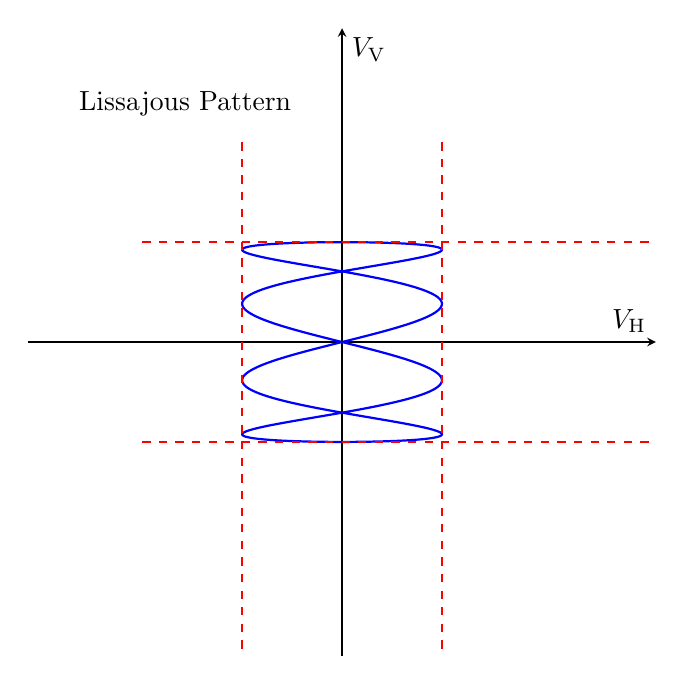
\begin{tikzpicture}
\begin{axis}[
    axis equal image,
    axis lines=center,
    xlabel={$V_\text{H}$},
    ylabel={$V_\text{V}$},
    xmin=-pi, xmax=pi,
    ymin=-pi, ymax=pi,
    xtick=\empty, ytick=\empty,
    trig format=rad,
    scale=1.4,
    title={Lissajous Pattern},
    title style={
        at={(axis cs:-pi/2,2)},
    }
]
    \addplot [thick, blue, domain=-pi:pi, samples=500] ({sin(4*x)}, {sin(x)});
    \draw[thick, red, dashed] (-1,2)--(-1,-pi);
    \draw[thick, red, dashed] (1,2)--(1,-pi);
    \draw[thick, red, dashed] (-2,1)--(pi,1);
    \draw[thick, red, dashed] (-2,-1)--(pi,-1);

\end{axis}
\end{tikzpicture}\hspace{5pt}\begin{tikzpicture}
\begin{axis}[
    axis equal image,
    axis lines=center,
    xmin=-pi, xmax=pi,
    ymin=-pi, ymax=pi,
    xtick=\empty, ytick=\empty,
    xlabel={$\omega t$},
    ylabel={$V_\text{V}$},
    xlabel style={above left},
    ylabel style={below right},
    trig format=rad,
    scale=1.4,
    title={$Y$ input},
    title style={
        at={(axis cs:-pi/2,2)},
    }
]
    \addplot [thick, blue, domain=-pi:pi, samples=500] {-sin(x)};
    \draw[thick, red, dashed] (-pi,1)--(-pi/2,1);
    \draw[thick, red, dashed] (-pi,-1)--(pi/2,-1);
\end{axis}
\end{tikzpicture}

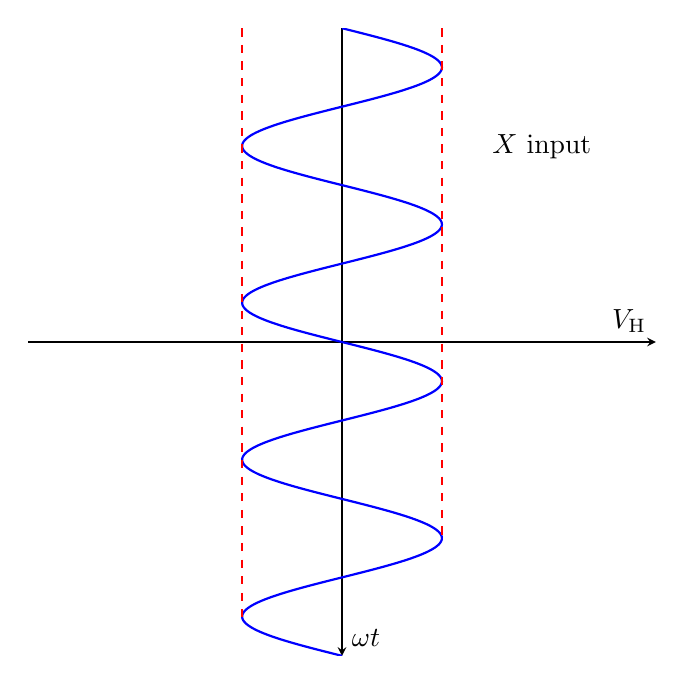
\begin{tikzpicture}
\begin{axis}[
    axis equal image,
    rotate around={-pi/2:(0,0)},
    axis lines=center,
    xmin=-pi, xmax=pi,
    ymin=-pi, ymax=pi,
    xtick=\empty, ytick=\empty,
    xlabel={$\omega t$},
    ylabel={$V_\text{H}$},
    xlabel style={above right},
    ylabel style={above left},
    trig format=rad,
    scale=1.4,
    title={$X$ input},
    title style={
        at={(axis cs:-pi/2,2)},
    }
]
    \addplot [thick, blue, domain=-pi:pi, samples=500] {sin(4*x)};
    \draw[thick, red, dashed] (-pi,1)--(5*pi/8,1);
    \draw[thick, red, dashed] (-pi,-1)--(7*pi/8,-1);
\end{axis}
\end{tikzpicture}

\begin{center}Axes in all graphs have the same scale and the same length.\end{center}

\textbf{2.4} The signals $V_1$ and $V_2$ are applied to the $X$ and $Y$ inputs of the scope. Sketch the Lissajous pattern and calculate the phase difference between the two signals.
\[V_1=10\cos(\omega t),\qquad V_2=15\sin(\omega t-180^\circ)\]

\textbf{Answer}: $V_1=10\cos(\omega t)=10\sin(\omega t+90^\circ)$

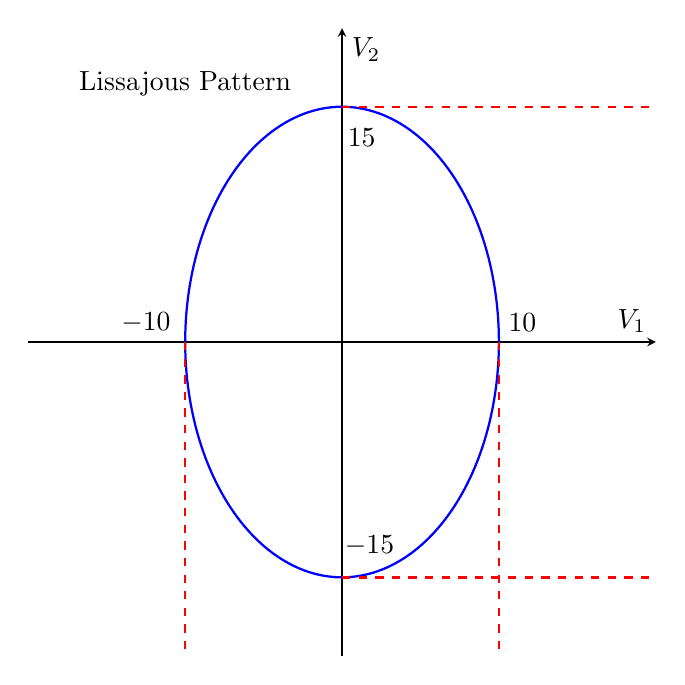
\begin{tikzpicture}
\begin{axis}[
    axis lines=center,
    axis equal image,
    xlabel={$V_1$},
    ylabel={$V_2$},
    xmin=-20, xmax=20,
    ymin=-20, ymax=20,
    xtick=\empty, ytick=\empty,
    trig format=rad,
    scale=1.4,
    title={Lissajous Pattern},
    title style={
        at={(axis cs:-10,14)},
    }
]
    \addplot [thick, blue, domain=-15:15, samples=500] ({10*cos(x-pi)},{15*sin(x)});
    \draw[thick, red, dashed] (0,-15)--(20,-15);
    \draw[thick, red, dashed] (0,15)--(20,15);
    \draw[thick, red, dashed] (-10,0)--(-10,-20);
    \draw[thick, red, dashed] (10,0)--(10,-20);
    \node at (1.25, 13) {$15$};
    \node at (11.5, 1.25) {$10$};
    \node at (1.75, -13) {$-15$};
    \node at (-12.5, 1.25) {$-10$};
\end{axis}
\end{tikzpicture}\hspace{5pt}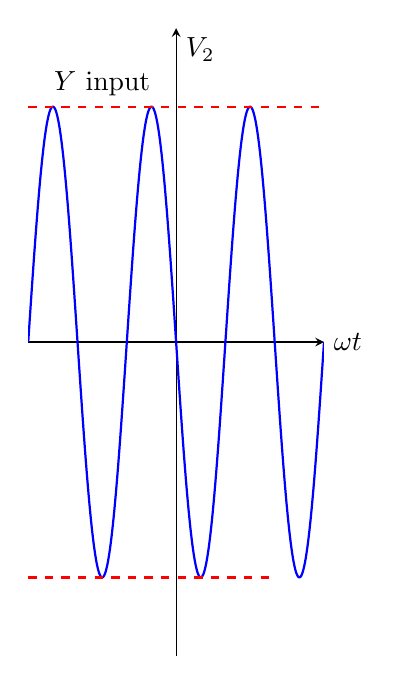
\begin{tikzpicture}
\begin{axis}[
    axis equal image,
    axis lines=center,
    xmin=-3*pi, xmax=3*pi,
    ymin=-20, ymax=20,
    xtick=\empty, ytick=\empty,
    xlabel={$\omega t$},
    ylabel={$V_2$},
    xlabel style={right},
    ylabel style={below right},
    trig format=rad,
    scale=1.4,
    title={$Y$ input},
    title style={
        at={(axis cs:-3*pi/2,14)},
    }
]
    \addplot [thick, blue, domain=-3*pi:3*pi, samples=500] {15*sin(x-pi)};
    \draw[thick, red, dashed] (-3*pi, 15) -- (3*pi, 15);
    \draw[thick, red, dashed] (-3*pi,-15) -- (2*pi,-15);
\end{axis}
\end{tikzpicture}

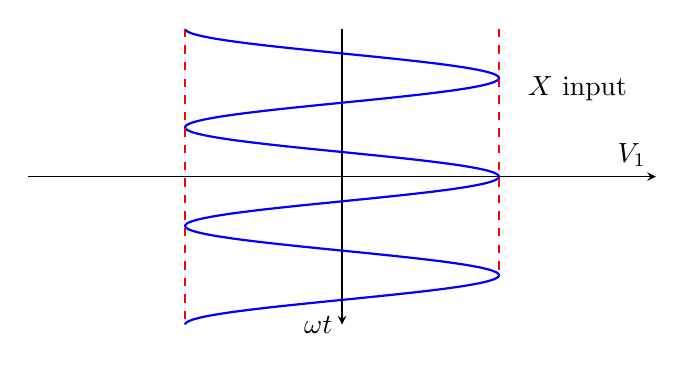
\begin{tikzpicture}
\begin{axis}[
    rotate around={-pi/2:(0,0)},
    axis equal image,
    axis lines=center,
    xmin=-3*pi, xmax=3*pi,
    ymin=-20, ymax=20,
    xtick=\empty, ytick=\empty,
    xlabel={$ \omega t$},
    ylabel={$V_1$},
    xlabel style={left},
    ylabel style={above left},
    trig format=rad,
    scale=1.4,
    clip=false,
    title={$X$ input},
    title style={
        at={(axis cs:-pi,15)},
    },
]
    \addplot [thick, blue, domain=-3*pi:3*pi, samples=500] {10*cos(x)};
    \draw[thick, red, dashed] (-3*pi,10)--(2*pi,10);
    \draw[thick, red, dashed] (-3*pi,-10)--(3*pi,-10);
\end{axis}
\end{tikzpicture}

\hfill

Phase angle: $90^\circ-(-180^\circ)=270^\circ$.

\end{document}